\section{Vorgänger Projekte}
\setauthor{Raffeiner Christine}
Die zwei folgenden Vorgängerprojekte wurden für die vorliegende Arbeit als Inspirationsquelle verwendet.
\begin{enumerate}
    \item \href{https://github.com/htl-leonding-project/questionz}{QuestionZ} \cite{noauthor_fragebogen_nodate}
    \item \href{https://github.com/htl-leonding-project/leo-survey}{Leo-survey} \cite{noauthor_fragebogen_nodate-1}
\end{enumerate}
QuestionZ ist ein Projekt bestehend aus Frontend, Backend und Datenbank und 
somit der Systemarchitektur der vorliegenden Arbeit sehr ähnlich.
Das Frontend von QuestionZ wurde jedoch mit JavaServerFaces (JSF) implementiert und war im Betrieb nicht stabil. 
Obwohl JSF immer noch weiterentwickelt wird, ist es für Neuprojekte oft nicht die erste Wahl, insbesondere wenn keine 
JavaEE bzw. JakartaEE-Backend verwendet wird. Das Backend von QuestionZ wurde in JavaEE mit einem Application
Server umgesetzt. JavaEE existiert mittlerweile nicht mehr und wurde von JakartaEE abgelöst. \cite{noauthor_fragebogen_nodate}
\newline
Leo-survey, der Namensvetter der Diplomarbeit, besteht im Gegensatz dazu aus einem Angular Frontend und einem Java 
Backend. Für die Datenbank wurde Derby gewählt. \cite{noauthor_fragebogen_nodate-1}
\newline
\newline
Leo-survey wurde mit Programmiersprachen implementiert, mit denen das Team vertraut war. Grundlegende Ideen zur 
Herangehensweise der Implementierung einiger Funktionen im Backend und Ideen für Layout und Design für die Entwicklung des 
Frontends wurden aus den Vorgängerprojekten geschöpft.
Aus dem Projekt QuestionZ entstand die erste stabile Version des Klassendiagramms. 

\section{Online Fragebogenwerkzeuge}
\setauthor{Raffeiner Christine}
Für eine Konkurrenzanalyse und Überlegungen, wie die vorliegende Arbeit von anderen 
Produkten abzugrenzen ist, wurden eine Reihe von Online-Fragebogen-Webseiten getestet und analysiert.
Weiters wurden interessante Funktionen und ansprechende Designideen gesammelt. Dabei wurde beachtet, dass  
die Arbeit hauptsächlich für den schulinternen Gebrauch gedacht ist. 

Dies ist eine Auflistung der Webseiten, die analysiert wurden:
\begin{itemize}
    \item 2ask.com \cite{noauthor_fragebogen_nodate-2}
    \item appinio.com \cite{noauthor_fragebogen_nodate-3}
    \item ingress.com \cite{noauthor_fragebogen_nodate-4}
    \item questionpro.com \cite{noauthor_fragebogen_nodate-5}
    \item survio.com \cite{noauthor_fragebogen_nodate-6}
    \item umfrageonline.com \cite{noauthor_fragebogen_nodate-7}
\end{itemize}

\subsection{2ask.com}
Dieses Tool bietet ähnliche Funktionen zu den Anforderungen der Arbeit, weshalb sie als Referenzobjekt sehr geeignet ist.
Besonderes Augenmerk wurde auf die Funktionen \textit{Fragebogen erstellen}, \textit{Umfragen durchführen} und \textit{Ergebnisse auswerten} gelegt.
Aufgefallen sind dabei die Erstellung eines QR-Codes, um Umfragen auszufüllen, der 
Datenexport der Auswertung in ein CSV-File und die Visualisierung der Auswertung mit 
verschiedenen Diagrammtypen. Negativ anzumerken ist, dass dieses Tool sehr viele Fragetypen besitzt, die die 
Erstellung eines Fragebogens verkomplizieren. \cite{noauthor_fragebogen_nodate-2}
\newline
Vorhandene Fragetypen sind:
\begin{itemize}
    \item Beschreibung
    \item Textfeld
    \item Formular
    \item Multiple-Choice
    \item Matrix
    \item Gruppen-Matrix
    \item Schieberegler (Sterne)
    \item Rangliste (Hierarchie)
    \item Konstantsummen
\end{itemize}

\begin{figure}[H]
    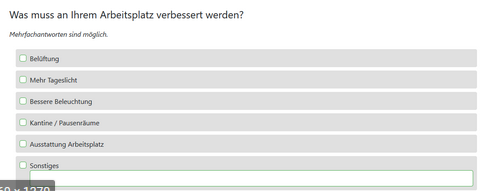
\includegraphics[width=0.8\textwidth]{pics/2ask_com.PNG}
    \centering
    \caption{Multiple-Choice-Frage von \cite{noauthor_fragebogen_nodate-2} }
    \label{fig:umfeld1}
\end{figure}

Von Interesse für designtechnische Aspekte ist die Angabe von sonstigen Antwortoptionen (siehe Abb. \ref{fig:umfeld1})
in Multiple-Choice-Fragen. Dieses Funktion deckt die Möglichkeit ab, dass keine der angegebenen Optionen für den 
Benutzer oder die Benutzerin in Frage kommt und optional eigene Antwortmöglichkeiten verwendet werden können. 
\newline
Ein tolles Feature für die Implementierung in die vorliegende Arbeit wäre die automatische Konvertierung 
sonstiger Optionen in vordefinierte Antwortmöglichkeiten. Umsetzen könnte man diese Konvertierung mittels algorithmischer Berechnungen.

\subsection{appinio.com}
Bei der Analyse dieses Tools stellte sich heraus, dass es sehr viele Funktionen beinhaltet. Die Auswertung liefert 
sehr ausführliche und mit vielen Details gespickte Informationen. Weiters ergab sich, dass das Tool für den Rahmen 
der Arbeit zu aufwendig gestaltet ist.

\begin{figure}[H]
    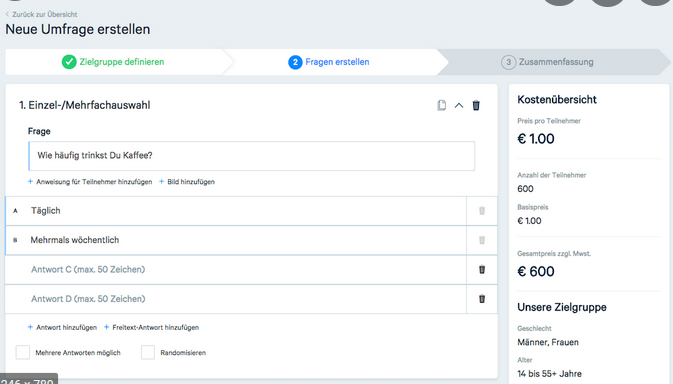
\includegraphics[width=0.8\textwidth]{pics/Appino_SteppsBeiErstellen.PNG}
    \centering
    \caption{Beispiel für die Erstellung eines Fragebogen von \cite{noauthor_fragebogen_nodate-3} }
    \label{fig:umfeld2}
\end{figure}

Das Design (siehe Abb. \ref{fig:umfeld2}) des Prozesses der Erstellung von Fragebogen ist sehr übersichtlich und optisch 
ansprechend umgesetzt. \cite{noauthor_fragebogen_nodate-3}

\subsection{ingress.com}
Das Tool Ingress deckt den Umfang der Arbeit mit seinen Funktionen ab. Mit ihm lassen sich Fragebögen erstellen, beantworten und auswerten. 
Während des Beantwortungsprozesses stellt Ingress ein Dashboard zur Verfügung, um den derzeitigen Stand der Umfrage zu überwachen.

\begin{figure}[H]
    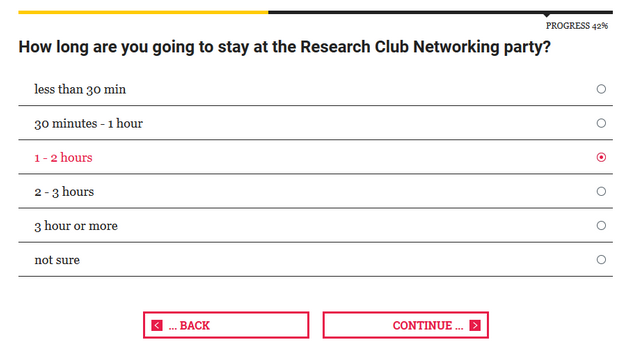
\includegraphics[width=0.8\textwidth]{pics/Ingress.PNG}
    \centering
    \caption{Fortschrittsanzeige bei der Beachtung der Fragebögen von \cite{noauthor_fragebogen_nodate-4} }
    \label{fig:umfeld3}
\end{figure}

Hervorzuheben bei diesem Tool ist die Fortschrittsanzeige, die während der Beantwortung von Umfragen (siehe Abb. \ref{fig:umfeld3}) angezeigt wird. 
Sie gibt den Benutzern eine direkte Rückmeldung über den Fortschritt und den Restaufwand, der betrieben werden muss, um 
das Ausfüllen des Fragebogens zu beenden. \cite{noauthor_fragebogen_nodate-4}

\subsection{questionpro.com}
Dieses Tool zeichnet sich durch das Analysieren der Daten in Echtzeit, die große Auswahl an Auswertungsdiagrammen und die 
resultierende genaue Auswertung aus. 

\begin{figure}[H]
    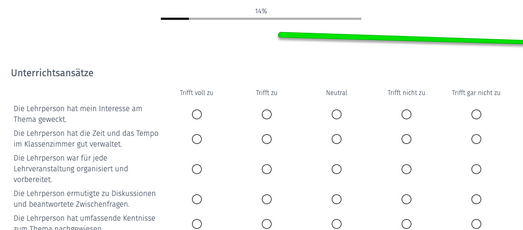
\includegraphics[width=0.8\textwidth]{pics/QuestionPro_Fortschrittsanzeige.PNG}
    \centering
    \caption{Fortschrittsanzeige bei der Beachtung der Fragebögen und Antwortoptionendesign von \cite{noauthor_fragebogen_nodate-5} }
    \label{fig:umfeld4}
\end{figure}

Dieses Tool bietet eine Fortschrittsanzeige, um Benutzerinnen und Benutzern eine direkte Rückmeldung über ihren derzeitigen Fortschritt zu geben.
(siehe Abb. \ref{fig:umfeld4}). Designtechnisch ist das Layout der Antwortoptionen von Interesse, da Optionen anders als 
Vergleichsobjekte nebeneinander statt untereinander angezeigt werden. Die Möglichkeit, diese Optionen nebeneinander 
anzuzeigen, ist nur dann sinnvoll, wenn die Optionen für jede Frage unverändert bleiben. Sollte das nicht der Fall sein, 
kann dadurch die Übersicht verloren gehen, da über jeder Antwortmöglichkeit ein anderer Text steht. \cite{noauthor_fragebogen_nodate-5}

\subsection{survio.com}
Bei diesem Tool war besonders das Herunterladen der Ergebnisse der Umfragen in vielen Formaten, beispielweise: PDF, DOCX, 
XLSX, CSV einprägsam.
\newline
\newline
Designtechnisch wurde auf die Verwendung von Radiobuttons verzichtet und stattdessen eine 
Auswahloption verwendet. Diese Option bietet dieselbe Funktionalität wie Radiobuttons, der / die Benutzer/in erkennt jedoch nicht 
auf den ersten Blick, welche Antwortmöglichkeiten die Frage hat. \cite{noauthor_fragebogen_nodate-6}

\subsection{umfrageonline.com}
Dieses Tool wurde genauer unter die Lupe genommen und es folgen die Erkenntnisse, die über das Design und die Funktionalitäten 
geschlossen wurden.

\begin{figure}[H]
    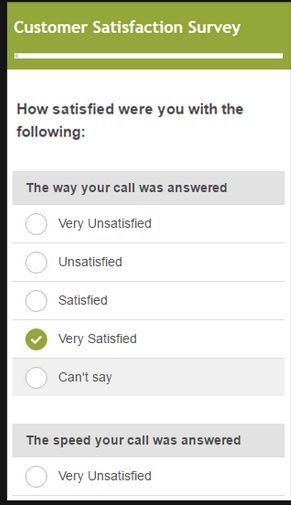
\includegraphics[width=0.3\textwidth]{pics/umfrageonline_com2.PNG}
    \centering
    \caption{Visuelle Trennung der Fragen von den Antwortoptionen von \cite{noauthor_fragebogen_nodate-7} }
    \label{fig:umfeld5}
\end{figure}

Das Tool zeigt (siehe Abb. \ref{fig:umfeld5}) eine visuelle Abtrennung von Fragen und Antwortmöglichkeiten, 
die hilft, nicht den Überblick bei einer großen Anzahl an Fragen und Antwortmöglichkeiten zu verlieren. 
Zudem dient es dazu, den Blick des Benutzers auf die Fragen zu fokussieren.
\begin{figure}[H]
    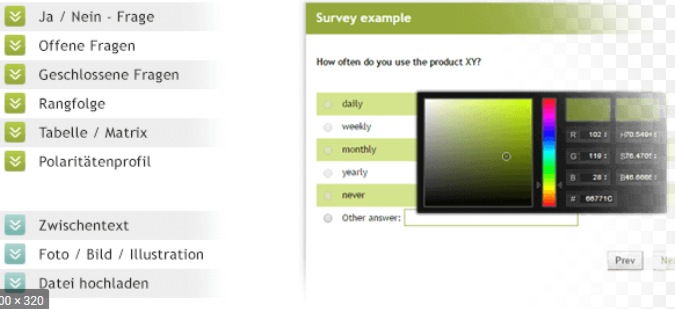
\includegraphics[width=0.8\textwidth]{pics/umfrageonline_com_erstellen.PNG}
    \centering
    \caption{Anpassung und Dateien zu einer Frage von \cite{noauthor_fragebogen_nodate-7} }
    \label{fig:umfeld6}
\end{figure}

Bilder oder Dateien, die zum Beantworten einer Frage nötig sind, zu einer Frage abzuspeichern, ist 
eine Funktionalität, die ein Fragebogentool von einem Anderen unterscheiden und abheben kann. Zudem ist die Funktion praktisch,
um wichtige Informationen zur Frage bereitzustellen. (siehe Abb. \ref{fig:umfeld6} als Beispiel). 
Den Umfang der Arbeit betrachtend, ist die in der Abbildung gezeigte Anpassung von Farben zu jedem Fragebogen zu aufwendig. 
Weiters wurden die Fragetypen analysiert. Die Implementierung aller Typen würde 
den Umfang der Arbeit überschreiten.

\begin{figure}[H]
    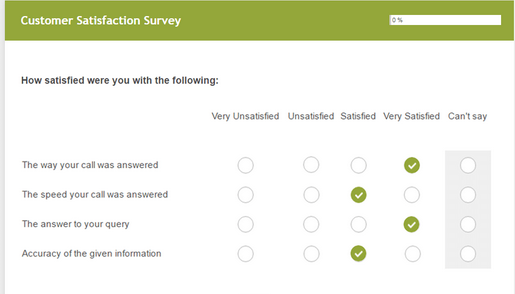
\includegraphics[width=0.8\textwidth]{pics/Umfrageonline_com_BlockanFragen.PNG}
    \centering
    \caption{Antwortoptionendesign von \cite{noauthor_fragebogen_nodate-7} }
    \label{fig:umfeld7}
\end{figure}

Dieses Tool bietet die Möglichkeit Antwortoptionen nebeneinander darzustellen.(siehe Abb. \ref{fig:umfeld7}). \cite{noauthor_fragebogen_nodate-7}, \cite{noauthor_pdflatex_nodate}